\documentclass[a4paper,11pt]{article}
% Various packages
\usepackage{siunitx}
\usepackage[utf8]{inputenc} % æøå
\usepackage[T1]{fontenc} % mere æøå
\usepackage[danish]{babel} % orddeling
\usepackage{verbatim} % så man kan skrive ren tekst
\usepackage{graphicx}
\graphicspath{{assets/}}
\usepackage{a4wide}
\usepackage{url}
\usepackage[left=2cm,top=2cm,bottom=1.5cm,right=2cm]{geometry}
\usepackage{amsmath}
\usepackage{amssymb}
\usepackage{amsthm}
\usepackage{wrapfig}
\usepackage{fixme}
\usepackage{color}
\usepackage{pstricks}
\usepackage{pdfpages} % include pdf
\usepackage{float} % Use [H] in figures
\usepackage{subcaption} % For subfigures
\usepackage{color} % May be necessary if you want to color links
\usepackage{hyperref} % Make references clickable
\usepackage[nameinlink,capitalize]{cleveref} % Make eq:refs be in style (1)
\usepackage[linesnumbered, commentsnumbered, lined, ruled, vlined,
%noend  % Have no ⌊-like symbol to indicate end of scope in pseudocode
]{algorithm2e} % Doc: https://goo.gl/6bC1qZ

% Ændr på navnene der vises når man bruger \autoref{label}
\def\sectionautorefname{Sektion}
\renewcommand{\equationautorefname}{Ligning}
\def\figureautorefname{Figur}
\AtBeginDocument{\renewcommand{\ref}[1]{\autoref{#1}}}

% Sæt \ref{} til at kalde \autoref{}
\AtBeginDocument{\renewcommand{\ref}[1]{\autoref{#1}}}

% Ændr ''*'' i math-felter til \cdot
\DeclareMathSymbol{*}{\mathbin}{symbols}{"01}

% Sæt farver for interne referencer og links
\definecolor{darkblue}{RGB}{25,25,112}
\hypersetup{
	colorlinks=true,    %set true if you want colored links
	linktoc=all,        %set to all if you want both sections and subsections linked
	linkcolor=darkblue, %choose some color if you want links to stand out
	filecolor=blue,     %
	citecolor=black,    %
	urlcolor=cyan,      %
}

% Set indentation to 0:
\setlength\parindent{0pt}

% Keywords relateret til algorithm2e pakken
\newcommand{\True}{\textbf{true}}\newcommand{\False}{\textbf{false}}
\SetStartEndCondition{ }{}{}%
\SetKwProg{Fn}{def}{\string:}{}
\SetKw{KwTo}{to}
\SetKwFor{For}{for}{}{}% 
\SetKwFor{ForEach}{foreach}{}{}% 
\SetKwIF{If}{ElseIf}{Else}{if}{}{elif}{else}{end}% 
\SetKwFor{While}{while}{}{end}\SetKwProg{Fn}{}{}{}
\SetKwInOut{Input}{input}\SetKwInOut{Output}{output}
\setlength{\algomargin}{3em}\DontPrintSemicolon

\newcommand{\longspace}{{\ \ \ \ \ \ \ \ \ \ \ \ \ \ }}
\renewcommand{\P}{{\mathbb P}}
\newcommand{\parfrac}[1]{\frac{\partial}{\partial #1}}
\renewcommand{\num}{{\textrm{num} }}
\newcommand{\size}{{\textrm{size} }}
\newcommand{\ift}{{\textrm{if } }}

% Dynamiske (), <>, ceil, floor
\newcommand{\p}[1]{\left( #1 \right)}
\newcommand{\pbig}[1]{\big( #1 \big)}
\newcommand{\pBig}[1]{\Big( #1 \Big)}
\newcommand{\pbigg}[1]{\bigg( #1 \bigg)}
\newcommand{\larr}[1]{\left< #1 \right>}
\newcommand{\ceil}[1]{\left\lceil #1 \right\rceil}
\newcommand{\floor}[1]{\left\lfloor #1 \right\rfloor}


% Squiggly arrows
\DeclareFontFamily{U} {MnSymbolC}{}

\DeclareFontShape{U}{MnSymbolC}{m}{n}{
	<-6> MnSymbolC5
	<6-7> MnSymbolC6
	<7-8> MnSymbolC7
	<8-9> MnSymbolC8
	<9-10> MnSymbolC9
	<10-12> MnSymbolC10
	<12-> MnSymbolC12}{}
\DeclareFontShape{U}{MnSymbolC}{b}{n}{
	<-6> MnSymbolC-Bold5
	<6-7> MnSymbolC-Bold6
	<7-8> MnSymbolC-Bold7
	<8-9> MnSymbolC-Bold8
	<9-10> MnSymbolC-Bold9
	<10-12> MnSymbolC-Bold10
	<12-> MnSymbolC-Bold12}{}

\DeclareSymbolFont{MnSyC} {U} {MnSymbolC}{m}{n}

\DeclareMathSymbol{\MNrhd}{\mathbin}{MnSyC}{76}
\DeclareMathSymbol{\MNlhd}{\mathbin}{MnSyC}{78}
% =============================================
\DeclareFontFamily{U} {MnSymbolD}{}

\DeclareFontShape{U}{MnSymbolD}{m}{n}{
	<-6> MnSymbolD5
	<6-7> MnSymbolD6
	<7-8> MnSymbolD7
	<8-9> MnSymbolD8
	<9-10> MnSymbolD9
	<10-12> MnSymbolD10
	<12-> MnSymbolD12}{}
\DeclareFontShape{U}{MnSymbolD}{b}{n}{
	<-6> MnSymbolD-Bold5
	<6-7> MnSymbolD-Bold6
	<7-8> MnSymbolD-Bold7
	<8-9> MnSymbolD-Bold8
	<9-10> MnSymbolD-Bold9
	<10-12> MnSymbolD-Bold10
	<12-> MnSymbolD-Bold12}{}

\DeclareSymbolFont{MnSyD} {U} {MnSymbolD}{m}{n}
\DeclareMathSymbol{\MNsim}{\mathbin}{MnSyD}{2}

% =============================================

\usepackage{amssymb,amsmath,stackengine}
\stackMath
\newcommand\rsquigarrow[1]{%
	\mathbin{\stackon[2pt]{\rightsquigarrow}{\scriptscriptstyle #1 }}
}

\author{Søren Mulvad, rbn601}

\title{Eksamensdisposition - Minimum Spanning Trees (MST)}
\begin{document}
\maketitle

% Desuden skal hver studerende i gruppen udarbejde en individuel disposition for emnet "Binære søgetræer", som er et af emnerne til eksamen. En disposition skal bestå af de vigtigste punkter, du vil komme ind på til eksamen.
% Tænk på dispositionen som noget, du kan have med dig til eksamen, og som kan hjælpe dig med at huske, hvad du overordnet vil gennemgå til emnet "Binære søgetræer".
% Dispositionen skal ikke indeholde detaljerede beviser og lignende, men de mere overordnede delemner. Sørg for at gøre den kortfattet - f.eks. 5-10 punkter med stikord/-sætninger.


\begin{itemize}
\item \textbf{Motivation samt beskrivelse af problemet}


\item \textbf{Generisk løsning}
\begin{itemize}
	\item Terminologi: Cut, krydse et cut, respektere et sæt $A$ af kanter, light kant, sikker kant.
\end{itemize}

\item \textbf{Bevis af Theorem 23.1 (Genkendelse af sikre kanter)}

\item \textbf{Håndkørsel af Kruskals algoritme}

\item \textbf{Håndkørsel af Prims algoritme}


\end{itemize}

%%%%%%%%%%%%%%%%%%%%%%%%%%%%%%%%%%%%%%%%%%%%%%%%%%%%%%%%%%%
%%%%%%%%%%%%%%%%%%%%%%%%%%%%%%%%%%%%%%%%%%%%%%%%%%%%%%%%%%%
%%%%%%%%%%%%%%%%%%%%%%%%%%%%%%%%%%%%%%%%%%%%%%%%%%%%%%%%%%%
\newpage
%%%%%%%%%%%%%%%%%%%%%%%%%%%%%%%%%%%%%%%%%%%%%%%%%%%%%%%%%%%
%%%%%%%%%%%%%%%%%%%%%%%%%%%%%%%%%%%%%%%%%%%%%%%%%%%%%%%%%%%
%%%%%%%%%%%%%%%%%%%%%%%%%%%%%%%%%%%%%%%%%%%%%%%%%%%%%%%%%%%
\section{Minimum Spanning Trees}



\begin{itemize}
\item \textbf{Motivation samt beskrivelse af problemet}
\begin{itemize}
	\item Løser det problem at forbinde en graf af knuder med den minimale omkostning.
	\item Bliver ofte benyttet til f.eks. at designe elektriske kredsløb.
	\item Kan modelleres som en graf $G = (V, E)$ hvor $V$ er sættet af knuder og $E$ er sættet af kanter. For hver kant $(u, v) \in E$ skal der være en vægtfunktion $w(u, v)$ som siger hvad omkostningen er.
	\item Vi vil gerne finde det acyklise subset $T \subseteq E$ som forbinder alle knuderne, og minimerer den totale vægt.
	\item Tegn en graf her hvor du beskriver terminologien ud fra, følgende er en god størrelse:
	\begin{center}
		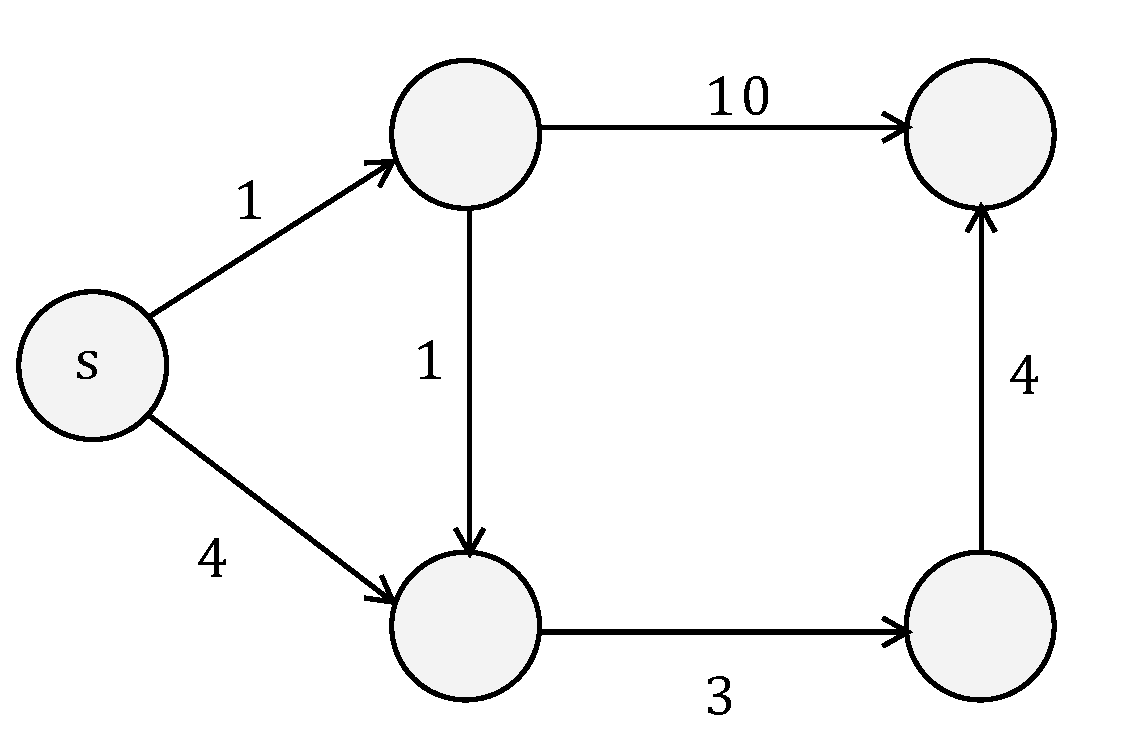
\includegraphics[width=0.4\textwidth]{graph.pdf}
	\end{center}
\end{itemize}


\item \textbf{Generisk løsning}
\begin{itemize}
	\item Terminologi:
	\begin{itemize}
		\item Cut: En partitionering $(S, V-S)$ af $V$ i grafen $G = (V, E)$. Vil sige at vi deler grafen op i to subsets.
		\item Krydse et cut: Når en kant $(u, v)$ kryder cuttet $(S, V-S)$ er det fordi en af endepunkterne er i $S$ og den anden er i $V-S$.
		\item Respektere et sæt $A$ af kanter: Når et cut ikke resulterer i, at nogle af kanterne i sættet $A$ krydser cuttet.
		\item Light kant: En kant, som både kryder et cut og hvis vægt er minimum af alle de kanter der kryder cuttet (NB: Der kan være flere for en iteration).
		\item Sikker kant: En kant vi kan tilføje til subsettet $A$, som vedligeholder at $A$ stadig er et subset af et Minimum Spanning Tree
	\end{itemize}
	\item Algoritme:\\
	\begin{algorithm}[H] \caption{Generic-MST} \label{alg:mst-gen}
		\SetKwFunction{func}{Generic-MST}%
		\Fn(){\func{G, w}}{
			$A = \emptyset$\;
			\While{$A \neq$ et Spanning Tree}{
				find en kant $(u, v)$ sikker for $A$\;
				$A = A \cup \{(u, v)\}$\;
			}
			\Return $A$\;
		}
	\end{algorithm}\vspace{1em}

	\item Trivielt ser vi, at for hver iteration vil $A$ være et subset af et MST da der kun tilføjes sikre kanter, og når algoritmen slutter er alle kanter tilføjet til $A$ i et MST.
\end{itemize}


\item \textbf{Bevis af Theorem 23.1 (Genkendelse af sikre kanter)}
\begin{itemize}
	\item \textit{Def:} For grafen $G = (V, E)$ med vægtfunktion $w$ defineret for $E$, så lad $A$ være et subset af $E$ som er inkluderet i et MST. Lad $(S, V-S)$ være ethvert cut af $G$ som respekterer $A$, og lad $(u,v)$ være en light kant der krydser dette cut.\\
	Så er kanten $(u, v)$ sikker for $A$.
	\item Lad os nu sige at vi har et Minimum Spanning Tree $T$, som også inkluderer subsettet $A$, og antage at $T$ ikke indeholder light kanten $(u, v)$.
	\item \textit{Mål:} Vi konstruerer nu et nyt MST $T'$ som inkluderer $A \cup \{(u, v)\}$ ved at bruge en cut-and-paste teknik, hvorved vi viser at $(u, v)$ er en sikker kant for $A$.
	 \begin{figure}[H]
	 	\begin{center}
	 		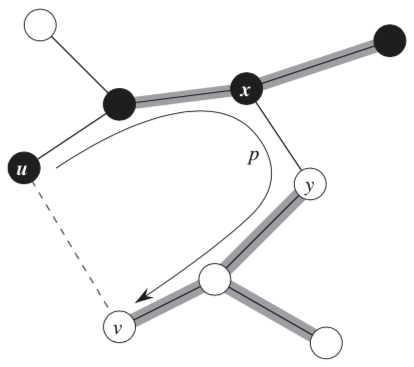
\includegraphics[width=0.4\textwidth]{mst.png}
	 	\end{center}
	 	\caption{Sorte knuder i $S$, hvide knuder i $V-S$. Kanterne i MST'et $T$ er vist, men ikke alle kanter i grafen $G$ er vist. Kanterne i $A$ er markeret og $(u,v)$ er en light kant der krydser cuttet $(S, V-S)$.}
	 	\label{fig:mst}
	 \end{figure}
 	\item Vi laver nu et cut $(S, V-S)$ som respekter subsettet $A$.
 	\item Kanten $(u, v)$ danner en cyklus med kanterne på den simple vej $p$ fra $u$ til $v$ i $T$, som set på \ref{fig:mst}.
 	\item Siden $u$ og $v$ er på modsatte sider af cuttet $(S, V-S)$, så må minimum en af kanterne i $T$ være på den simple vej $p$ og samtidig krydse cuttet. Lad os kalde den kant $(x, y)$.
 	\item Kanten $(x, y)$ er ikke i $A$, siden cuttet respekterer $A$.
 	\item Da vi har at $(x, y)$ er en del af den unikke simple vej fra $u$ til $v$, så vil det at fjerne den skære $T$ over i to komponenter.
 	\item Tilføjer vi nu $(u, v)$ genforbinder vi komponenterne og får et nyt spanning tree
 	$$
 	T' = T + \{(u, v)\} - \{(x, y)\}
 	$$
 	\item Herefter skal vi vise at $T'$ er et Minimum Spanning Tree. Siden $(u, v)$ er en light kant der kryder $(S, V-S)$ og $(x, y)$ også krydser dette cut, så får vi:
 	\begin{align*}
 	w(T') &= w(T) + \overbrace{w(u, v) - w(x, y)}^{\text{$\leq 0$ da $w(u, v) \leq w(x, y)$}}\\
 	      &\leq w(T)
 	\end{align*}
 	Men vi havde før defineret $T$ til at være et minimum spanning tree, så vi har også $w(T) \leq w(T')$, altså må $T'$ også være et MSP.
 	\item Vi skal stadig vise at $(u, v)$ faktisk er en sikker kant for $A$.\\
 	Da $A \subseteq T$ og $(x, y) \notin A$ må vi have at $A \subseteq T'$. Derfor må også $A \cup \{(u, v)\} \subseteq T'$.\\
 	Siden $T'$ er et minimum spanning tree må der gælde, at $(u, v)$ er en sikker kant for $A$.
\end{itemize}


\newpage
\item \textbf{Håndkørsel af Kruskals algoritme}
\begin{itemize}
	\item Grådig algoritme \textit{(Skriv ikke op, men for forståelse under forberedelse)}:\\
	\begin{algorithm}[H] \caption{MST-Kruskal} \label{alg:kruskal}
		\SetKwFunction{func}{MST-Kruskal}%
		\SetKwFunction{MakeSet}{Make-Set}%
		\SetKwFunction{FindSet}{Find-Set}%
		\SetKwFunction{Union}{Union}%
		\Fn(){\func{G, w}}{
			$A = \emptyset$\;
			\ForEach{vertex $v \in G.V$}{
				\texttt{Make-Set}$(v)$\;
			}
			sort the edges of $G.E$ into increasing order by weight $w$\;
			\ForEach{edge $(u, v) \in G.E$ in sorted order}{
				\If{\FindSet{u} $\neq$ \FindSet{v}}{
					$A = A \cup \{(u, v)\}$\;
					\Union{u, v}\;
				}
			}
			\Return $A$\;
		}
	\end{algorithm}\vspace{1em}
	
	
	\item Altså:\\
	Start med et tomt sæt $A$\\
	Lav et nyt sæt for hver knude\\
	Sorter alle kanter efter stigende vægt $w$\\
	For hver eneste kant i sorteret rækkefølge, hvis de to knuder forbundet af kanten ikke er en del af samme sæt, så tilføj kanten til $A$ og foren de to knuder.
	\item Illustration:
	\begin{figure}[H]
		\begin{center}
			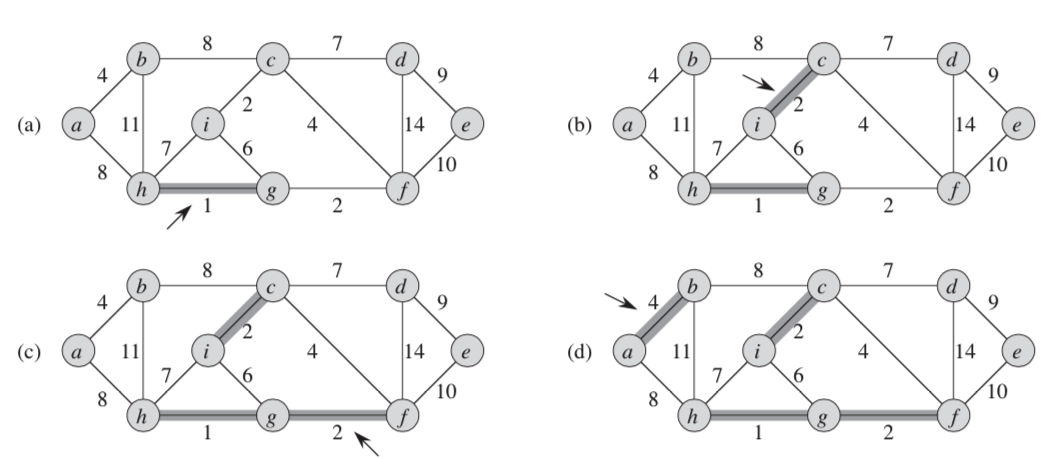
\includegraphics[width=0.7\textwidth]{kruskal.png}
		\end{center}
		\caption{Kruskals algoritme \textit{(fortsætter, kun første fire steps)}}
		\label{fig:kruskal}
	\end{figure}
	
	
	
	\item Køretiden afhænger af hvor hurtigt vi kan tjekke om to elementer er en del af samme sæt samt forene dem. Vi bruger disjoint set forests.\\
	
	Sortering af kanterne tager $O(E \lg E)$ tid. Efter det udfører vi $O(E)$ \texttt{Find-Set} og \texttt{Union}, som sammen med $|V|$ \texttt{Make-Set} operationer tager $O\pBig{(V+E) \ \alpha(V)}$-tid.\\
	$\alpha(V)$ er en funktion der vokser \textit{meget} langsomt\\
	
	Da vi antager at grafen er forbundet har vi $|E| \geq |V| - 1$, og derfor kan vi omskrive ovenstående til $O(E \alpha(V))$ tid.\\
	
	Vi har, at $\alpha(|V|) = O(\lg V) = O(\lg E)$, og derfor kan vi skrive køretiden fra det som $O(E \lg E) = O(E \lg V)$. Vi ser derfor, at algoritmen umiddelbart er upper-boundet af sorteringen.
	Da det er et MST vi skal finde, kan vi dog også antage, at det er en forbundet graf, hvorved $|E| \leq |V|^2$, så $\lg E = \lg V^2 = 2\lg V = O(\lg V)$. Derfor kan vi skrive den endelige køretid som:
	$$
	O(E \lg E) = O(E \lg V)
	$$
\end{itemize}



\newpage
\item \textbf{Håndkørsel af Prims algoritme}
\begin{itemize}
	\item Grådig algoritme
	\item Vi starter ved en rodknude $r$ og tilføjer herefter altid en light kant der krydser cuttet $(S, V-S)$. Har den effekt at vores subset $A$ hele tiden er et sammenhængende træ.
	\item Virker ved at holde styr på en $v.key$ og $v.\pi$ (parent-pointer) for alle knuder $v \in V$, som til at starte med sættes til henholdsvis $\infty$ og \texttt{NIL}. Herefter opdateres de omkringliggende kanter til den knude vi pt. kigger på såfremt værdierne er bedre.
	\item Illustration:
	\begin{figure}[H]
		\begin{center}
			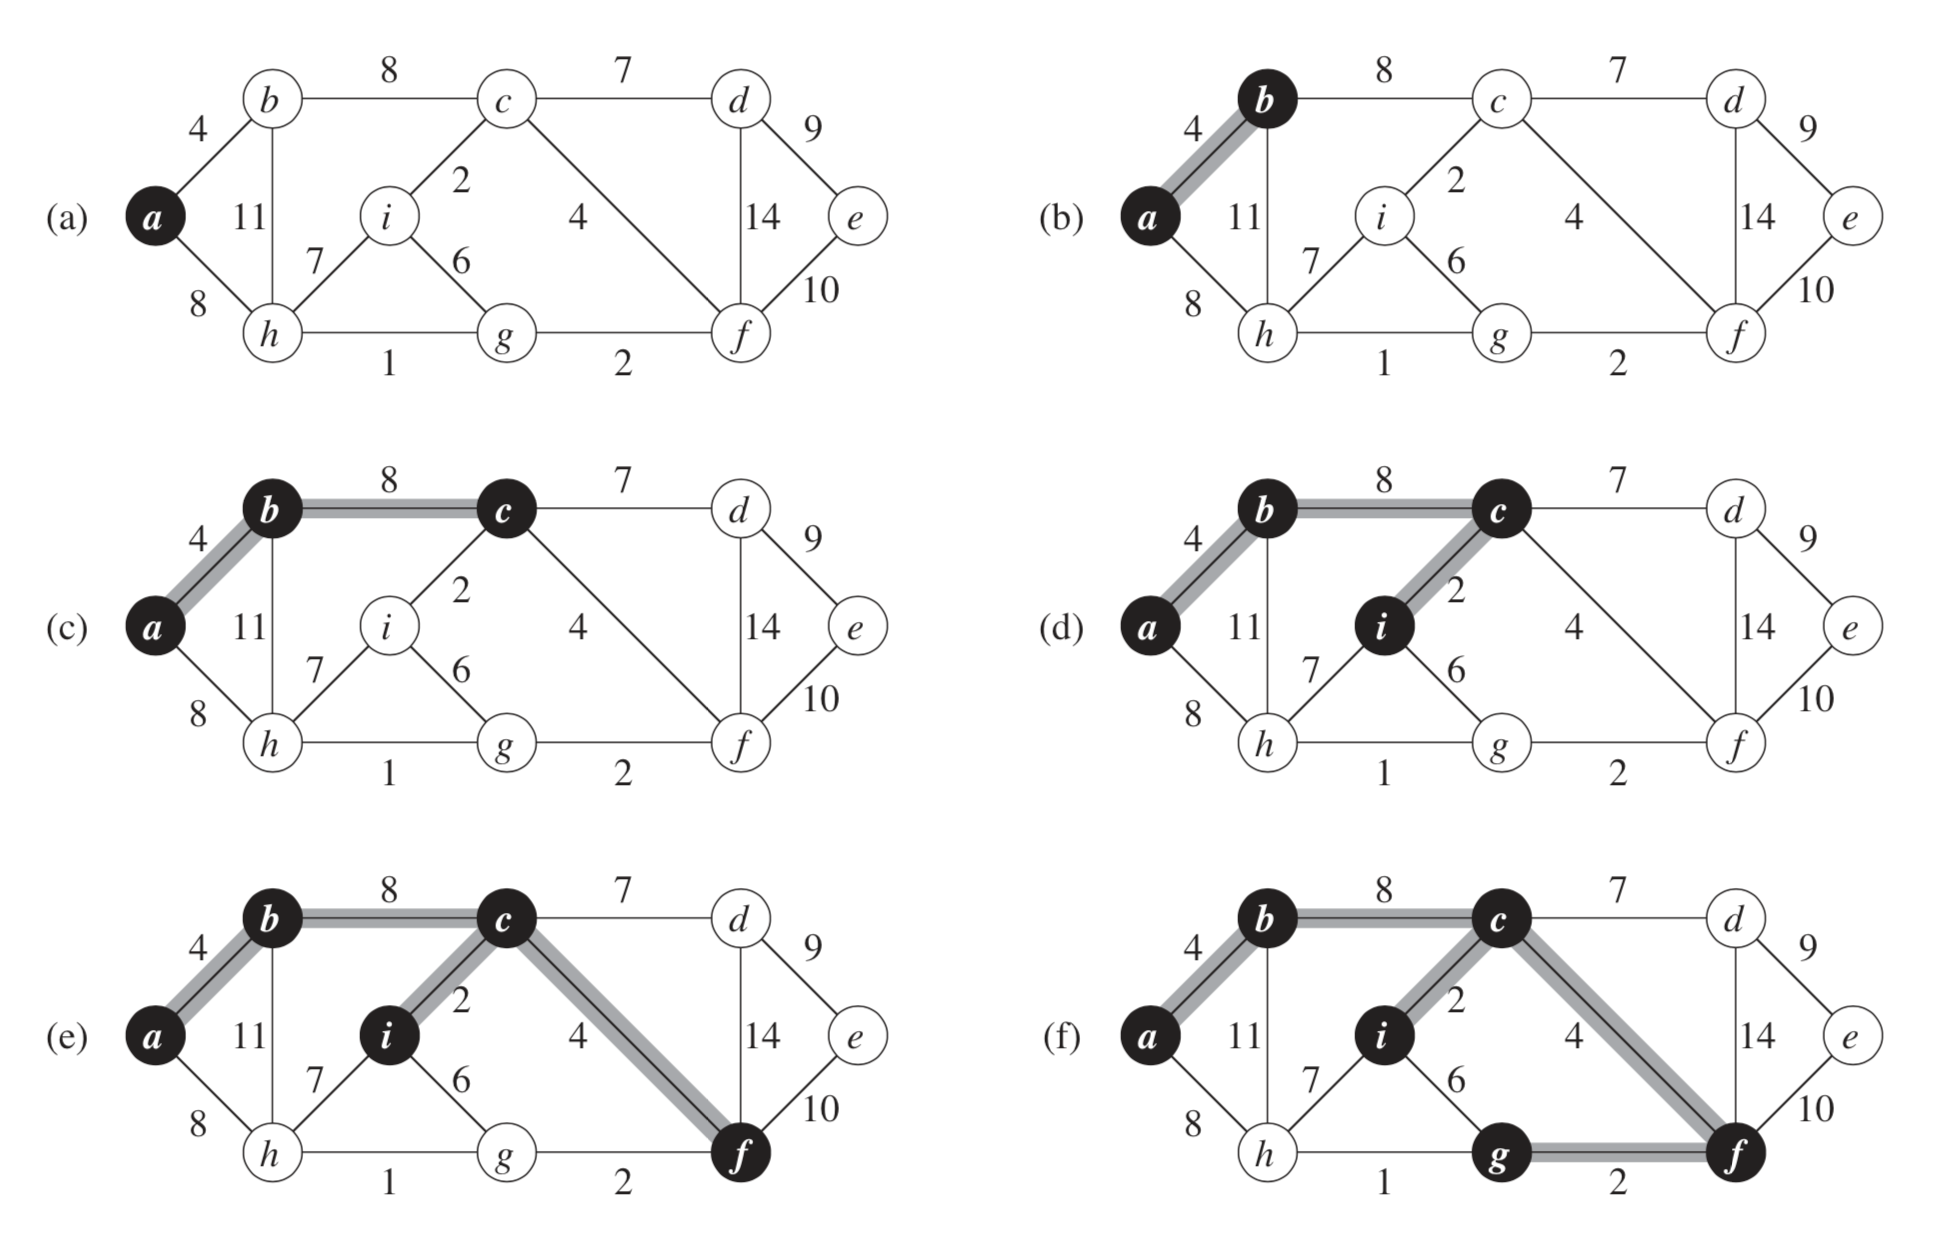
\includegraphics[width=\textwidth]{prim.png}
		\end{center}
		\caption{Prims algoritme \textit{(fortsætter, kun første seks steps)}.\\
			Bemærk at vi i step (b)-(c) både kunne have valgt enten kanten $(b, c)$ eller kanten $(a, h)$.}
		\label{fig:prim}
	\end{figure}
	\item Køretiden afhænger af hvor hurtigt vi kan køre \texttt{Extract-Min} og \texttt{Decrease-Key}. Derfor er det optimalt at bruge Fibonacci Heaps. Der er $|V|$ elementer at holde styr på, så hver \texttt{Extract-Min} operation vil tage $O(\lg n)$ amortiseret tid. Derudover udfører vi $2 |E|$ \texttt{Decrease-Key} operationer, som hver amortiseret tager $O(1)$ tid. Altså vil den totale køretid blive:
	$$
	O(V \lg V + E)
	$$
\end{itemize}



\end{itemize}
\end{document}